This chapter covers the details of the Single Chip Mote bootloader, the specialized hardware and software used to load compiled C code onto the instruction memory for the ARM Cortex-M0. The bootloader requires four distinct hardware/software components:

\begin{description}
	\item[Instruction ROM on Single Chip Mote] This is a read-only memory located in the \texttt{AHBIMEM} module. This ROM contains the basic software, referred to from now on as firmware, that runs on the ARM Cortex-M0 while the main software is loaded into the instruction RAM.
	\item[Instruction RAM on Single Chip Mote] This is a synchronous SRAM located in the \texttt{AHBIMEM} module to hold the main software for the Single Chip Mote. This RAM has no valid data when the FPGA is powered on, and must be loaded with the right software through bootloading. This RAM is written either from the ARM Cortex-M0 via the AHB bus, or from external hardware using the 3 Wire Bus.
	\item[Bootload Hardware on Nexys 3] This is a custom FPGA project meant for the Digilent Nexys 3 board. The hardware in this project is designed to read software from the special programmable RAM on the Nexys 3 board and then transmit it over the 3 Wire Bus to another board, containing the Single Chip Mote digital system.
	\item[Bootload Firmware for ARM Cortex-M0] This is a small program C program for the ARM Cortex-M0, meant to perform any actions to assist the bootloading process. The end of this program resets the system and the code in the instruction RAM is executed.
\end{description}


\section{Reset Signals and Bootloading}
As shown in section \ref{PON}, the \texttt{PON} module samples an external reset signal and a reset request signal (\texttt{SYSRESETREQ}) from the ARM Cortex-M0, and generates two separate system-level resets for all other modules in the digital system. These are referred to as the hard reset and the soft reset. The hard reset is triggered when the external reset button is pressed (or upon power-up or bitstream loading). The soft reset is triggered by either the external reset button or the reset request signal from the Cortex-M0. Almost all modules in the digital system use the soft reset. However, the \texttt{AHBIMEM} module uses both the hard and soft reset signals for different registers. The purpose and functionality of these two resets in the \texttt{AHBIMEM} module are explained in the following section.

 \section{Instruction ROM on the Single Chip Mote}
The instruction ROM is a 16kB single-port ROM where instruction data is fetched after the system is initially powered-on (or in the case of an FPGA, when the bitstream is initially loaded). The \texttt{AHBIMEM} module contains a special register, called \texttt{imem\_mode}, to select between the instruction RAM and ROM for instruction fetches. The \texttt{imem\_mode} register has two resets, connected to the hard reset and the soft reset, and cannot be changed at any other time. The hard reset takes precedence over the soft reset, and sets \texttt{imem\_mode} to ROM. Thus the instructions in the ROM always execute after power-on, bitstream loading, or external reset. On a soft reset, the \texttt{imem\_mode} register is set to a  value stored in the \texttt{next\_imem\_mode} register. \texttt{next\_imem\_mode} must be set by the ARM Cortex-M0 prior to requesting a reset. This register is set by writing to the \texttt{BOOTLOADER\_REG\_\_CFG} register. The purpose of the firmware, executing from the ROM, is to perform any necessary preparations during bootloading, set the \texttt{next\_imem\_mode} register to RAM, and then send a reset request. After a soft reset, instructions are fetched and executed from the RAM.
 
 In an ASIC, ROM is considered to be hard-coded and cannot be changed after tapeout. However, on an FPGA, the value of this ROM is initialized using a COE file. See section \ref{instruction-ROM} for more information on initializing the ROM.
 
 \section{Instruction RAM on the Single Chip Mote}
 The instruction RAM is a 64kB dual-port RAM in where the main software for the ARM Cortex-M0 is stored and fetched during regular operation of the Single Chip Mote. This RAM is not connected to either of the two reset signals, and thus is unaffected by a system reset.
 
 The \texttt{AHBIMEM} module has two AHB slave interfaces, one only for reading instructions, and one for reading bootloading status and writing bootload configuration and data. The write port of this RAM is connected to a 3 Wire Bus interface and an AHB slave interface of the \texttt{AHBIMEM} for bootloading. The \texttt{boot\_mode} register in the \texttt{AHBIMEM} module determines whether the 3 Wire Bus, the AHB, or neither write to the RAM. This register is set to neither upon reset, and can be changed by the ARM Cortex-M0 by writing to the  \texttt{BOOTLOADER\_REG\_\_CFG} register. The read port of this RAM is connected to the AHB slave interface of the \texttt{AHBIMEM} for instruction data.
 
 \section{3 Wire Bus Interface} \label{3wb}
 The 3 Wire Bus (3WB) is an interface used to serially send instruction data from the bootload hardware (on a separate FPGA board) to the Single Chip Mote (either on an FPGA or an ASIC). The three wires for this bus are clock, data, and latch. This interface operates according to the following rules:
 
 \begin{itemize}
 	\item The data line is connected to a 31-bit shift register.
 	\item Data is shifted onto the shift register on each rising edge of the clock.
 	\item The latch signal is asserted just before the 32nd rising edge of the clock.
 	\item The latch signal causes the 31 bits in the shift register, and the signal on the data line (for 32 bits total) to be written into the instruction RAM, as long as the \texttt{boot\_mode} register is set to allow the 3 Wire Bus to write into the RAM.
 	\item The \texttt{AHBIMEM} module keeps track of the RAM write address, and increments this address on every write.
 	\item Once the instruction RAM has been filled (in this case 64kB of data has been written), the \texttt{AHBIMEM} module considers the boot finished and does not allow further writes from the 3 Wire Bus (unless the system is reset).
 \end{itemize}
 
 The \texttt{AHBIMEM} module implements the receiving end of this interface. The bootload hardware on the Nexys 3 implements the transmitting end of this interface.
 
\section{Bootload Hardware on Nexys 3}
The bootload hardware on the Digilent Nexys 3 board is used to copy the main software from a computer onto the RAM on the Nexys 3 board, and then send that data over the 3 Wire Bus interface. The ISE project file for this design is \path{scm-digital/proj/ise/spartan6/bootloader/BootloadHW.xise} and the source code is found in \path{scm-digital/src/hw/spartan6/bootloader/}.

This hardware contains two state machines and one 32kB FIFO. The first state machine reads 16 bits of data out of the Nexys 3 external RAM (referred to by Digilent as Cellular RAM) at 50MHz. The RAM is operated in a special burst mode, where one line of 128 16-bit words is read back-to-back at high frequencies. The state machine reads the data out of the RAM and writes it to the FIFO, pausing at the end of each 128-word line for two reasons: the first is to allow for a data refresh cycle in the RAM, and the second is to check and wait for the FIFO to have enough room for another 128 words of data. The second state machine reads 32 bits out of the FIFO at 5 MHz, and sends one bit at a time over the 3 Wire Bus interface.

The first state machine is activated by pressing the button on the Nexys 3 board labeled BTNU. Once 64kB of instruction data has been sent over the 3 Wire Bus interface, the LED on the Nexys 3 board labeled LED0 lights up. The unlabeled button in the center of the group of buttons resets the bootload hardware.

\section{Bootload Firmware for ARM Cortex-M0}
\subsection{Firmware Essentials}
The bootload firmware is a small program designed for facilitating the bootloading process using the ARM Cortex-M0 on the Single Chip Mote. The firmware can perform any function or use any peripheral just like the main software for the Single Chip Mote; however, it is limited to a size of 16kB and is permanently kept in ROM. Therefore it is essential that the firmware performs exactly what is needed, nothing more, and is absolutely correct. Regardless of how the new instruction data is received and loaded into the ROM, the firmware must perform two important functions in order to ensure that the main software is executed. The first is that the instruction memory is set to boot from RAM after a soft reset. The second, is to send a reset request after the bootloading has completed.

\subsection{Application Interrupt and Reset Control Register}
The Application Interrupt and Reset Control Register (AIRCR) is a status and reset control register for the ARM Cortex-M0. See ARM documentation for more details on this register. Setting the second bit of this register, the \texttt{SYSRESETREQ} bit, indicates a request for a system-level reset. This asserts the \texttt{SYSRESETREQ} signal in the hardware, and the \texttt{PON} module generates the soft reset in response.

\subsection{AHB Slave Interface for Bootloading}
The \texttt{AHBIMEM} module has a special AHB slave interface for bootloading. This interface is accessed using addresses with the prefix 0x01 (this includes any address in the range of 0x01000000 to 0x01FFFFFF). Any AHB reads to an address with the prefix 0x01 returns the read-only \texttt{BOOTLOADER\_REG\_\_STATUS} register contents. This register shows the current \texttt{imem\_mode}, \texttt{next\_imem\_mode}, and \texttt{boot\_mode} values. It also shows whether bootloading through the 3 Wire Bus has finished (as in 64kB of data has been written through the 3 Wire Bus). Any AHB write to an address in the range of 0x01000000 - 0x0100FFFF will result in a write into the instruction RAM at the corresponding address, with the prefix of 0x01 replaced with 0x00. Any AHB write to the address 0x01F00000 will result in a write to the write-only \texttt{BOOTLOADER\_REG\_\_CFG} register. Writing to this register sets \texttt{next\_imem\_mode} and \texttt{boot\_mode}. The table in Figure \ref{table:boot-reg-status} describes the bit fields in the read-only \texttt{BOOTLOADER\_REG\_\_STATUS} register, and the table in Figure \ref{table:boot-reg-cfg} describes the bit fields in the write-only \texttt{BOOTLOADER\_REG\_\_CFG} register.

\begin{figure}
\centering
\begin{tabular}{|c|c|c|}
	\hline
	Field Bits & Field Name & Possible Values \\
	\hline
	0 & \texttt{imem\_mode} & 0 = ROM, 1 = RAM \\
	1 & \texttt{next\_imem\_mode} & 0 = ROM, 1 = RAM \\
	3:2 & \texttt{boot\_mode} & 00 = 01 = NONE, 10 = 3WB, 11 = AHB \\
	4 & \texttt{boot\_3wb\_done} & 0 = 3WB boot not done, 1 = 3WB boot done \\
	31:5 & Unused & Unspecified \\
	\hline
\end{tabular}
\caption{Register fields for the read-only \texttt{BOOTLOADER\_REG\_\_STATUS} register}
\label{table:boot-reg-status}
\end{figure}

\begin{figure}
\centering
\begin{tabular}{|c|c|c|}
	\hline
	Field Bits & Field Name & Possible Values \\
	\hline
	1:0 & \texttt{boot\_mode} & 00 = 01 = NONE, 10 = 3WB, 11 = AHB \\
	2 & \texttt{next\_imem\_mode} & 0 = ROM, 1 = RAM \\
	\hline
\end{tabular}
\caption{Register fields for the write-only \texttt{BOOTLOADER\_REG\_\_CFG} register}
\label{table:boot-reg-cfg}
\end{figure}

\subsection{Bootloading with the 3 Wire Bus} \label{3wb-boot}
All firmware loading software via the 3 Wire Bus must follow the same basic procedure:

\begin{enumerate}
	\item Set the \texttt{boot\_mode} register to 3WB
	\item Poll the \texttt{BOOTLOADER\_REG\_\_STATUS} register until \texttt{boot\_3wb\_done} is 1
	\item Set the \texttt{boot\_mode} register to NONE
	\item Set the \texttt{next\_imem\_mode} register to RAM
	\item Set the \texttt{SYSRESETREQ} bit of the AIRCR to trigger a soft reset
\end{enumerate}

\subsection{Bootloading with the AHB Slave Interface}
The AHB slave interface for bootloading is typically used in situations where software data is sent over another interface accessible by the ARM Cortex-M0, such as the radio or UART.  In future iterations of the Single Chip Mote might also include an optical interface to send software data to multiple devices at once. All firmware used to load software via the AHB slave interface must follow the same basic procedure:

\begin{enumerate}
	\item Set the \texttt{boot\_mode} register to AHB
	\item Listen to the radio/UART/optical interface that is sending the instruction data
	\item Copy the instruction data one word at a time into the instruction ROM by writing to addresses with the \texttt{0x01} prefix
	\item Set the \texttt{boot\_mode} register to NONE
	\item Set the \texttt{next\_imem\_mode} register to RAM
	\item Set the \texttt{SYSRESETREQ} bit of the AIRCR to trigger a soft reset
\end{enumerate}

\subsection{Current Firmware Implementation}
The current implementation of the firmware is found in \path{scm-digital/proj/keil/firmware/bootloader.uvproj}. It follows the same process described in section \ref{3wb-boot}. The bootloader first prints a message over UART saying "Welcome to the Bootloader. Setting boot mode to 3WB." The \texttt{boot\_mode} register is changed to 3WB, and then the \texttt{BOOTLOADER\_REG\_\_STATUS} register is repeatedly polled until \texttt{boot\_3wb\_done} is 1. The \texttt{boot\_mode} is changed to NONE, and the \texttt{next\_imem\_mode} register is set to RAM. At that point another message is printed over UART says "Boot complete. Restarting...". There is a long, empty for loop in order to allow for the entire message to print, and then the \texttt{SYSRESETREQ} bit of the AIRCR is set.

\section{Loading Software Using the Bootloader} \label{loading-sw}
Loading software onto the Single Chip Mote requires three files:

\begin{itemize}
	\item The bitstream file for the Single Chip Mote digital system, \path{ucontroller.bit}. For the Nexys 4 DDR using the Artix-7, this bitstream is generated using the ISE project found at \path{scm-digital/proj/ise/artix7/SingleChipMote/SingleChipMote.xise}. For the Nexys 3 using the Spartan-6, this bitstream is generated using the ISE project file found at \path{scm-digital/proj/ise/spartan6/uRobotDigitalController/uRobotDigitalController.xise}. For more information on how to generate a bitstream file, see section \ref{synthesis-loading}.
	\item The bitstream file for the bootloading hardware, \path{top.bit}. This bitstream is generated using the ISE project found at \path{scm-digital/proj/ise/spartan6/bootloader/BootloadHW.xise}. For more information on how to generate a bitstream file, see section \ref{synthesis-loading}.
	\item The C binary file containing the software to be loaded, code.bin. This is compiled using the Keil uVision5 project found at \path{scm-digital/proj/keil/uRobotDigitalController/code.uvprojx}. For more information on how to build and compile the software, see section \ref{keil}.
\end{itemize}

Once these three files have been generated, the two FPGA boards must be connected to one another as well as connected to the computer via the micro-USB ports on the boards. It is also recommended that a serial terminal is used to read the UART output of the Single Chip Mote to verify that the firmware was loaded successfully.

\subsection{Connecting UART} \label{uart}
Only the FPGA board containing the Single Chip Mote digital system needs to be connected via UART. The bootload hardware does not use UART.

For the Nexys 4 DDR, connect the micro-USB port labeled PROG UART to the computer and move the power switch to the ON position. This USB port is used for both programming and UART communication. Once the board has been recognized by the computer and the proper drivers have been installed, use Device Manager to find the COM port associated with the Nexys 4 board. From here, open up any serial terminal program, and connect to the COM port associated with the Nexys 4 board using the following settings: baud rate of 19200, with 8 data bits, 1 stop bits, no parity bits, and no flow control. Load the bitstream file using the instructions in section \ref{synthesis-loading}. Once the Single Chip Mote bitstream file has been loaded onto the board, there will be a message sent over UART from the bootloader reading "Welcome to the Bootloader."

For the Nexys 3, connect the micro-USB port labeled UART to the computer and move the power switch to the ON position. This USB port is used only for UART and not for programming. Once the board has been recognized by the computer and the proper drivers have been installed, use Device Manager to find the COM port associated with the Nexys 3 board. From here, open up any serial terminal program, and connect to the COM port associated with the Nexys 3 board using the following settings: baud rate of 19200, with 8 data bits, 1 stop bits, no parity bits, and no flow control. Load the bitstream file using the instructions in section \ref{synthesis-loading}. Once the Single Chip Mote bitstream file has been loaded onto the board, there will be a message sent over UART from the bootloader reading "Welcome to the Bootloader."

\subsection{Using Nexys 3 to Load Nexys 4 DDR}
The following steps show how to load the Single Chip Mote hardware and software onto a Nexys 4 DDR board:

\begin{enumerate}
	\item The Nexys 3 and Nexys 4 DDR boards each use three ports on one of the Pmod connectors for the 3 Wire Bus. While the boards are powered off, connect port JB1 on the Nexys 4 to port JB1 on the Nexys 3, for the data wire. Connect port JB2 on the Nexys 4 to port JB7 on the Nexys 3, for the latch wire. Connect port JB10 on the Nexys 4 to port JB10 on the Nexys 3, for clock wire. Also connect the ground ports (JB5 or JB11) of the two boards together. See Figure \ref{fig:bootload-nexys4} for an image of this setup.
	\item On the Nexys 4 DDR, connect the micro-USB port labeled PROG UART to the computer.
	\item On the Nexys 3, connect the micro-USB port labeled USB PROG to the computer.
	\item Switch on both of the boards. Ensure that both boards are recognized and that all drivers are installed.
	\item Open a serial terminal program and connect to the COM port of the Nexys 4 DDR using the instructions in section \ref{uart}.
	\item Open Digilent Adept, and load the C binary file, code.bin, onto the external RAM of the Nexys 3. For more instructions on this process see section \ref{digilent-adept}.
	\item Use Digilent Adept to load the bootload hardware bitstream file, top.bit, onto the Nexys 3. For more instructions on this process, see section \ref{digilent-adept}.
	\item Open iMPACT, and load the bitstream file for the Single Chip Mote digital system onto the Nexys 4. For more instructions on this process, see section \ref{synthesis-loading}.
	\item From here a message will be sent over UART, reading "Welcome to the Bootloader. Setting boot mode to 3WB." The Single Chip Mote is now waiting for the software data to be sent over the 3 Wire Bus.
	\item Press the button labeled BTNU on the Nexys 3 board. The LED labeled LED0 will light up when all of the data has been sent. Another message will be sent over UART, reading "Boot complete. Restarting..."
	\item After a slight pause, the main software will load. This is indicated by a message sent over UART reading "Welcome to the uRobot Digital Controller. Initialization Complete."
\end{enumerate}

\begin{figure}
\centering
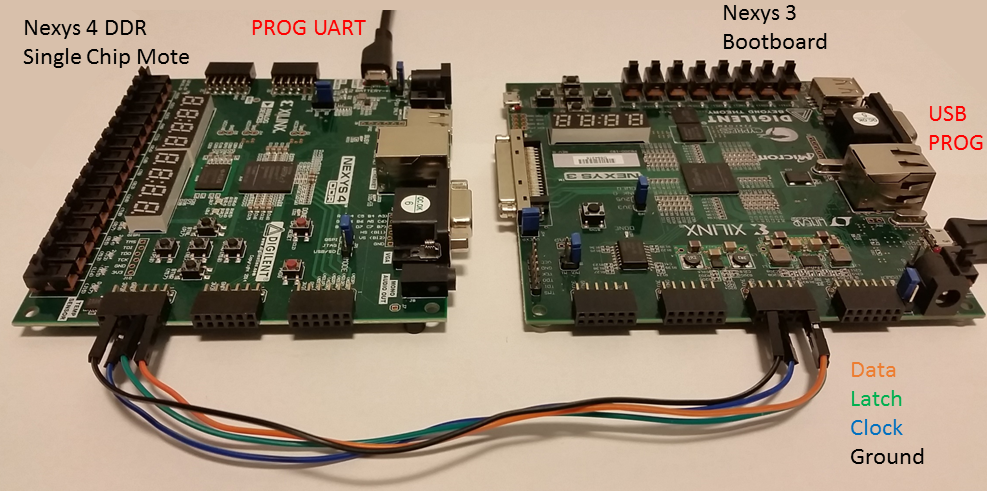
\includegraphics[width=1\linewidth]{bootload-nexys4}
\caption{Physical connections to load the Nexys 4 DDR with the Nexys 3}
\label{fig:bootload-nexys4}
\end{figure}

\subsection{Using Nexys 3 to Load Nexys 3}
Older versions of the Single Chip Mote digital system can also be loaded onto a Digilent Nexys 3 board instead of the Nexys 4 DDR. In this case, two Nexys 3 boards are required, one now referred to as the SCMboard and one now referred to as the bootboard. The SCMboard also needs a special expansion board from Digilent called the VmodMIB \cite{vmodmib-store}, as the 3 Wire Bus clock input is attached to one of the Pmod connectors on this expansion board.

To load the Single Chip Mote hardware and software on the SCMboard:

\begin{enumerate}
	\item The SCMboard and bootboard each use three ports on one of the Pmod connectors for the 3 Wire Bus. While the boards are powered off, connect port JB1 on the SCMboard to port JB1 on the bootboard, for the data wire. Connect port JB2 on the SCMboard to port JB7 on the bootboard, for the latch wire.
	\item Attach the VmodMIB expansion board to the SCMboard. Connect port JB10 on the VmodMIB to port JB10 on the bootboard, for clock wire. Also connect any of the ground ports of the two Nexys 3 boards together. See Figure \ref{fig:bootload-nexys3} for an image of this setup.
	\item On the SCMboard, connect the micro-USB port labeled USB PROG to the computer. Also connect the micro-USB port labeled UART to the computer.
	\item On the bootboard, connect the micro-USB port labeled USB PROG to the computer.
	\item Switch on both of the boards. Ensure that both boards are recognized and that all drivers are installed.
	\item Open a serial terminal program and connect to the COM port of the SCMboard using the instructions in section \ref{uart}.
	\item Open Digilent Adept, and load the C binary file, code.bin, onto the external RAM of the bootboard. For more instructions on this process see section \ref{digilent-adept}.
	\item Use Digilent Adept to load the bootload hardware bitstream file, top.bit, onto the bootboard. For more instructions on this process, see section \ref{digilent-adept}.
	\item Use Digilent Adept load the bitstream file for the Single Chip Mote digital system onto the SCMboard. For more instructions on this process, see section \ref{digilent-adept}.
	\item From here a message will be sent over UART, reading "Welcome to the Bootloader. Setting boot mode to 3WB." The Single Chip Mote is now waiting for the software data to be sent over the 3 Wire Bus.
	\item Press the button labeled BTNU on the bootboard board. The LED labeled LED0 will light up when all of the data has been sent. Another message will be sent over UART, reading "Boot complete. Restarting..."
	\item After a slight pause, the main software will load. This is indicated by a message sent over UART reading "Welcome to the uRobot Digital Controller. Initialization Complete."
\end{enumerate}

\begin{figure}
\centering
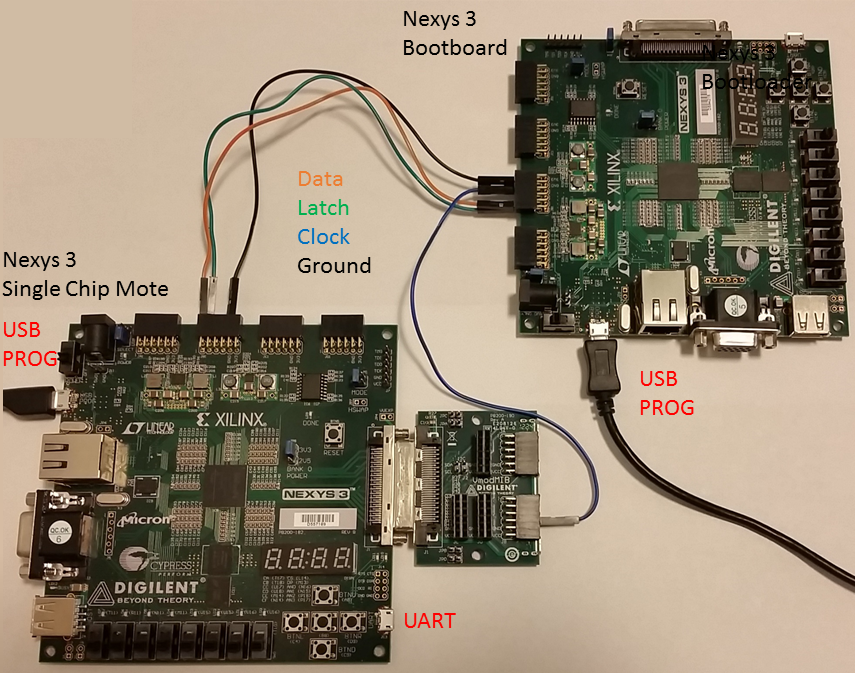
\includegraphics[width=1\linewidth]{bootload-nexys3}
\caption{Physical connections to load the Nexys 3 with another Nexys 3}
\label{fig:bootload-nexys3}
\end{figure}

\section{Connecting Two FPGA Boards for Simulated Packet Transmission} \label{connecting-two-boards}
The Single Chip Mote on both the Nexys 3 and Nexys 4 DDR do not have actual radios connected to the FPGAs. However, there are four GPIO pins on each board dedicated to simulating packet transmission, by connecting the transmitted data output (and its clock) of one board to the received data input (and its clock) of another, and vice versa. Note that the Nexys 4 DDR design uses the same pin for the received data clock and the 3 Wire Bus clock, and therefore the Nexys 4 DDR will need to be disconnected from the bootloading board.

The first step is to program each board with the Single Chip Mote hardware and software using the bootloader. Both boards should be connected to the computer via UART if commands to send and receive packets are given from the computer using UART. If the boards are programmed using the 3 Wire Bus, then the associated wires must be disconnected after programming.

The next step is to connect the ground pins of both boards to each other. On the Nexys 4 DDR, port JB11 can be used and on the Nexys 3, port JC5 can be used.

The next steps are to connect the \texttt{tx\_clk} pin of one board to the \texttt{rx\_clk} pin of the other board, and vice versa. Then connect the \texttt{tx\_dout} pin of one board to the \texttt{rx\_din} pin of the other board, and vice versa. On the Nexys 4 DDR, the \texttt{tx\_clk} pin is found on port JB7, the \texttt{tx\_dout} pin is found on port JB8, the \texttt{rx\_din} pin is found on port JB9, and the \texttt{rx\_clk} pin is found on port JB10. On the Nexys 3, the \texttt{rx\_clk} pin is found on port JC1, the \texttt{rx\_din} pin is found on port JC2, the \texttt{tx\_dout} pin is found on port JC3, and the \texttt{tx\_clk} pin is found on port JC4. Figure \ref{fig:connect-two-boards} shows two Nexys 4 DDR boards connected together.

Once the two boards are connected together, packets can be ``transmitted'' between the two boards without using a radio. This is done to verify that the radio controller hardware and software is working correctly.

\begin{figure}
	\centering
	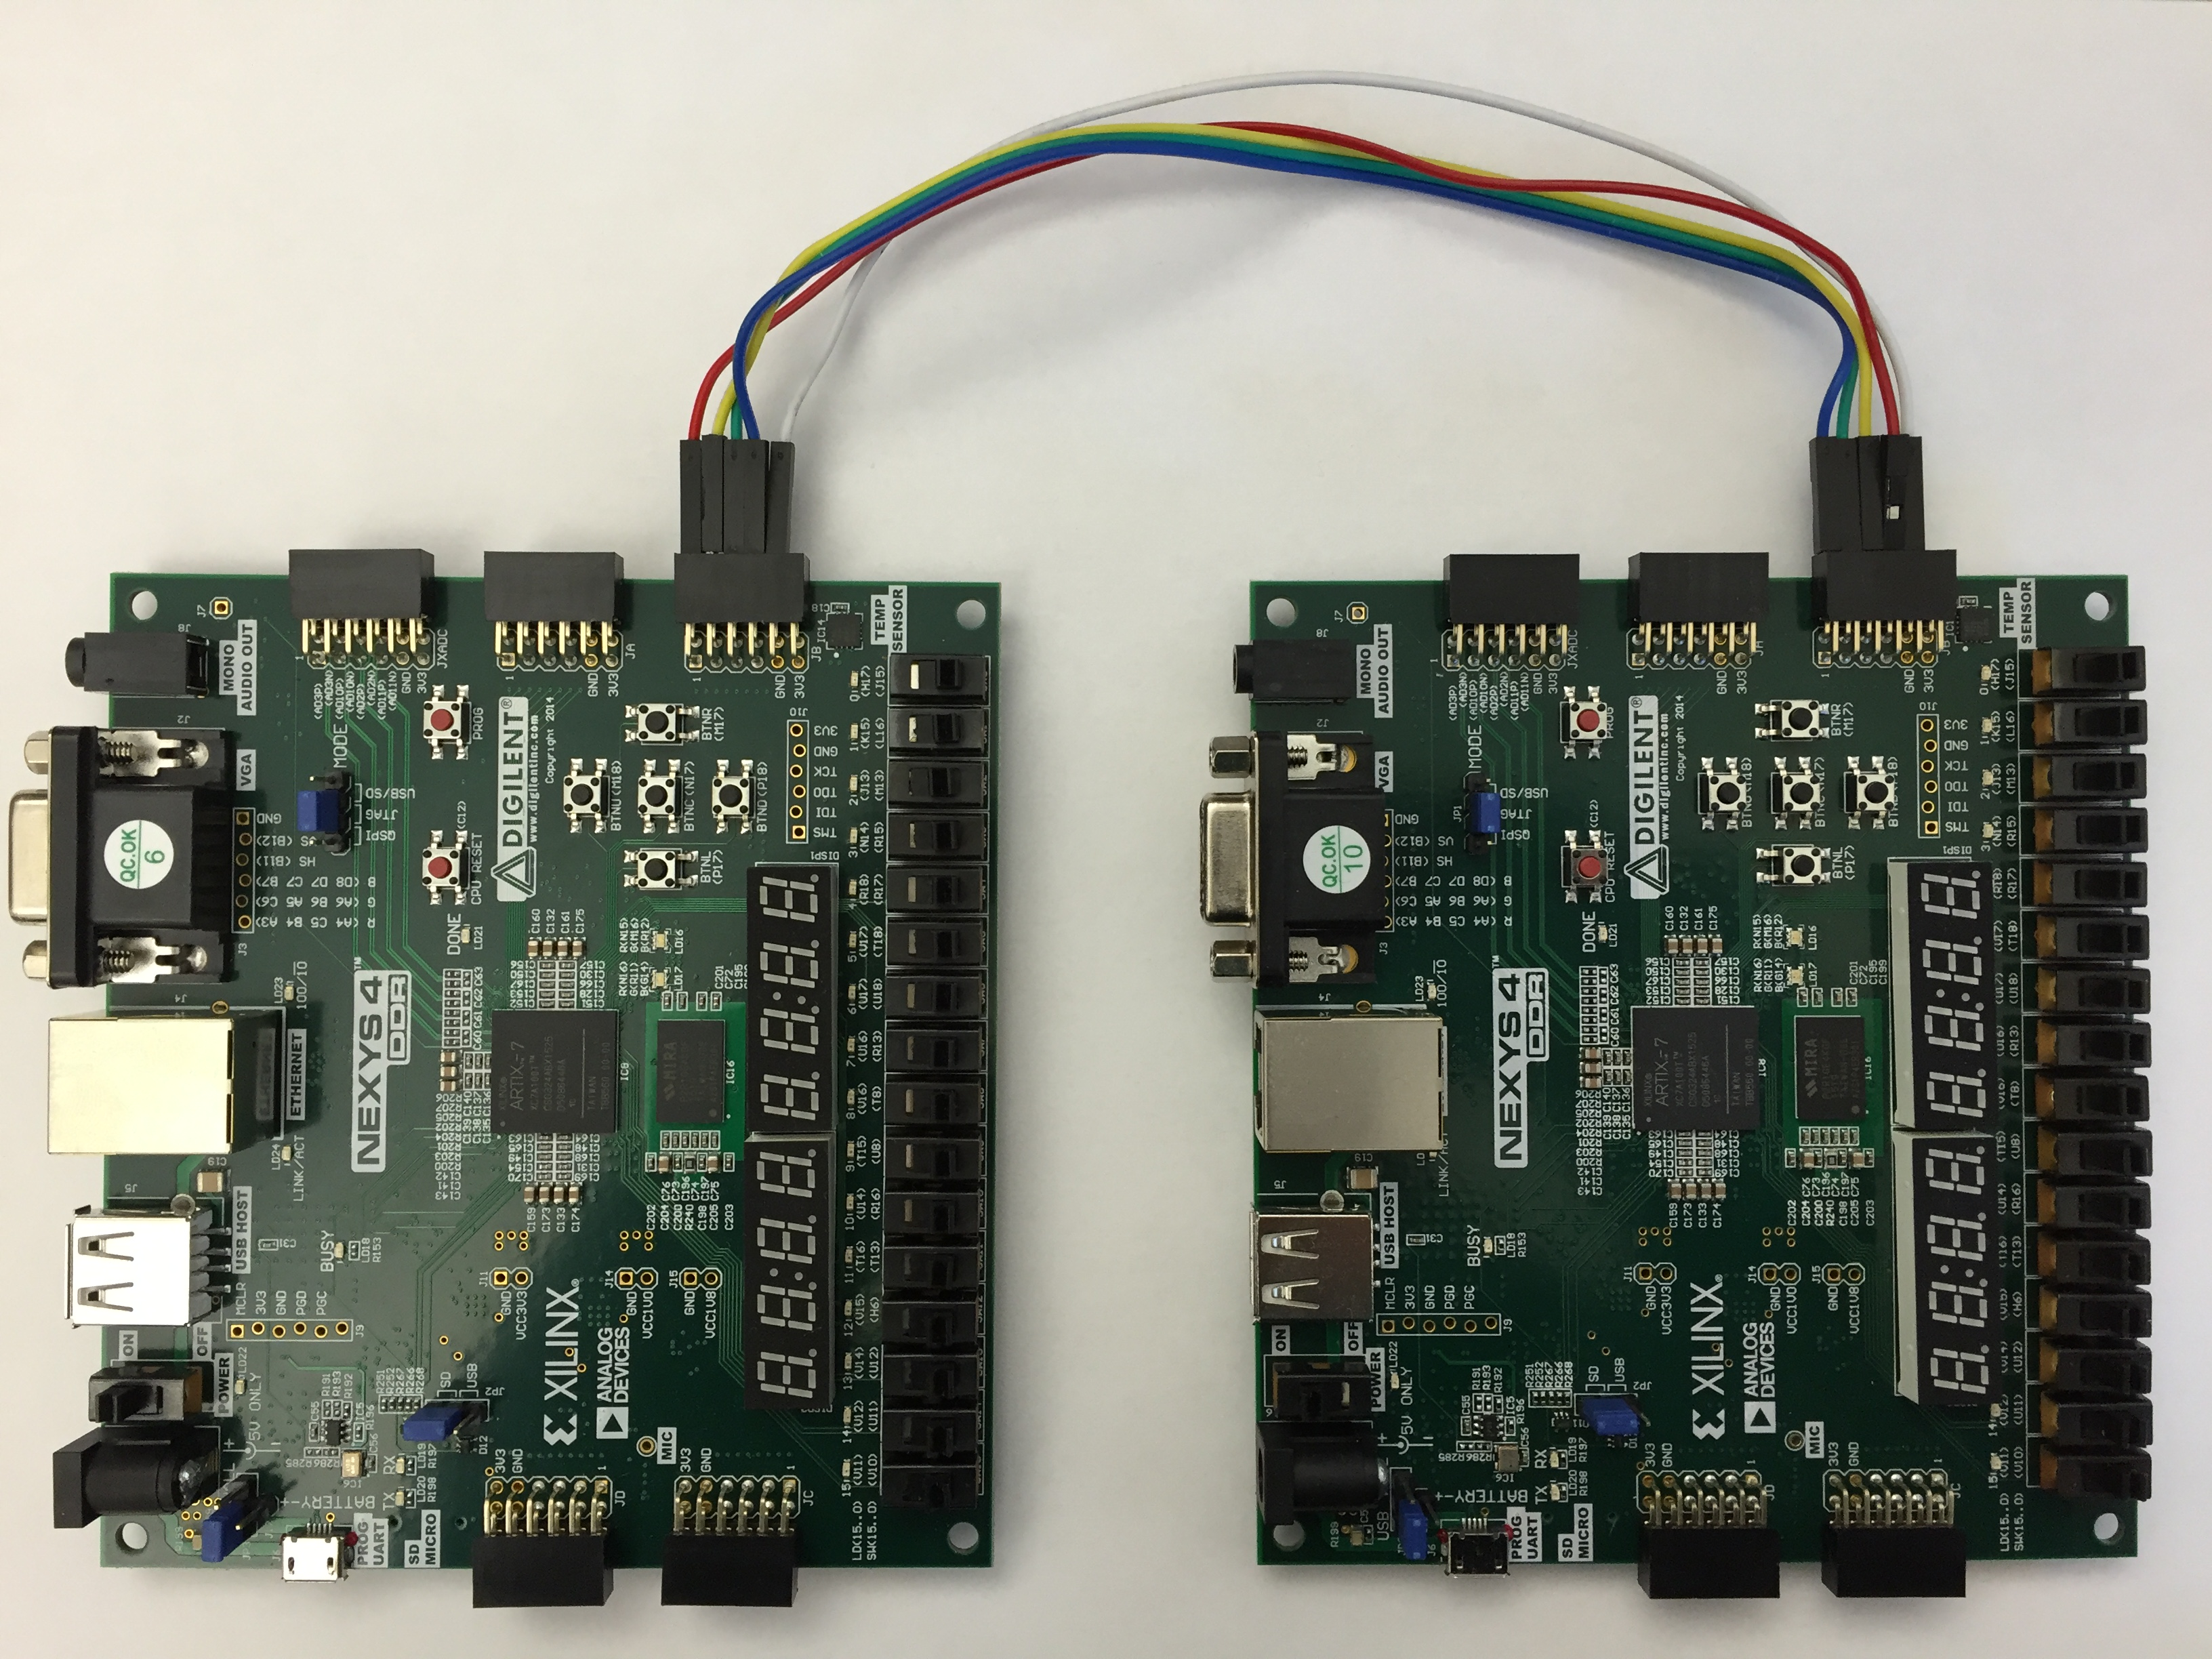
\includegraphics[width=1\linewidth]{connect-two-boards}
	\caption{Connecting two Nexys 4 DDR boards for simulated packet transmission without a radio}
	\label{fig:connect-two-boards}
\end{figure}
